\documentclass{article}

\usepackage{geometry}
\geometry{a4paper, scale=0.8}

\usepackage{graphicx}
\usepackage{float}

\usepackage{ctex}

\title{ISOA Final Report}
\author{Group "200"\\YiDai 2017013562\\ZhaohengLi 2017050025}

\begin{document}
\maketitle

\section{项目介绍}
我们以疫情部分的舆论方面为核心,提取舆论主题,结合时间线展示群众的关注点变化,对访问者提供舆论谣言判断服务。同时我们也注意到,信息服务平台如果缺失一方面的关键信息很容易丧失吸引力,我们还会实现政府的相关措施发布、并实现确诊数据展示。另外,我们引入了舆论用户评价功能以及疫情经济相关内容。

主要功能实现如下:
\begin{itemize}
	\item{\textbf{疫情展示}} 主要包括疫情确诊地图、详细数字和相关新闻或政策的时间线。
	\item{\textbf{舆情关注展示}} 收集各大网站新闻数据以及微博等社交平台舆论数据,对舆情进行主题提取,结合时间线展示群众的关注点变化
	\item{\textbf{虚假新闻/谣言判断及搜索}} 用户输入文本,对文本进行分析,为用户提供相关已证实谣言或者相关新闻,并给出用户输入文本为谣言的概率。
	\item{\textbf{用户评价舆论}} 将用户测试过的舆论信息以弹幕形式在页面中展示,并允许用户进行评价或者分享添加自己已知的信息,打造信息共享平台。
	\item{\textbf{疫情经济展示}} 展示疫情下股市的走动以及相关的新闻动态。同时允许用户设置一些提醒规则,如价格下行突破5日均线。
\end{itemize}

\begin{figure}[H]
\centering
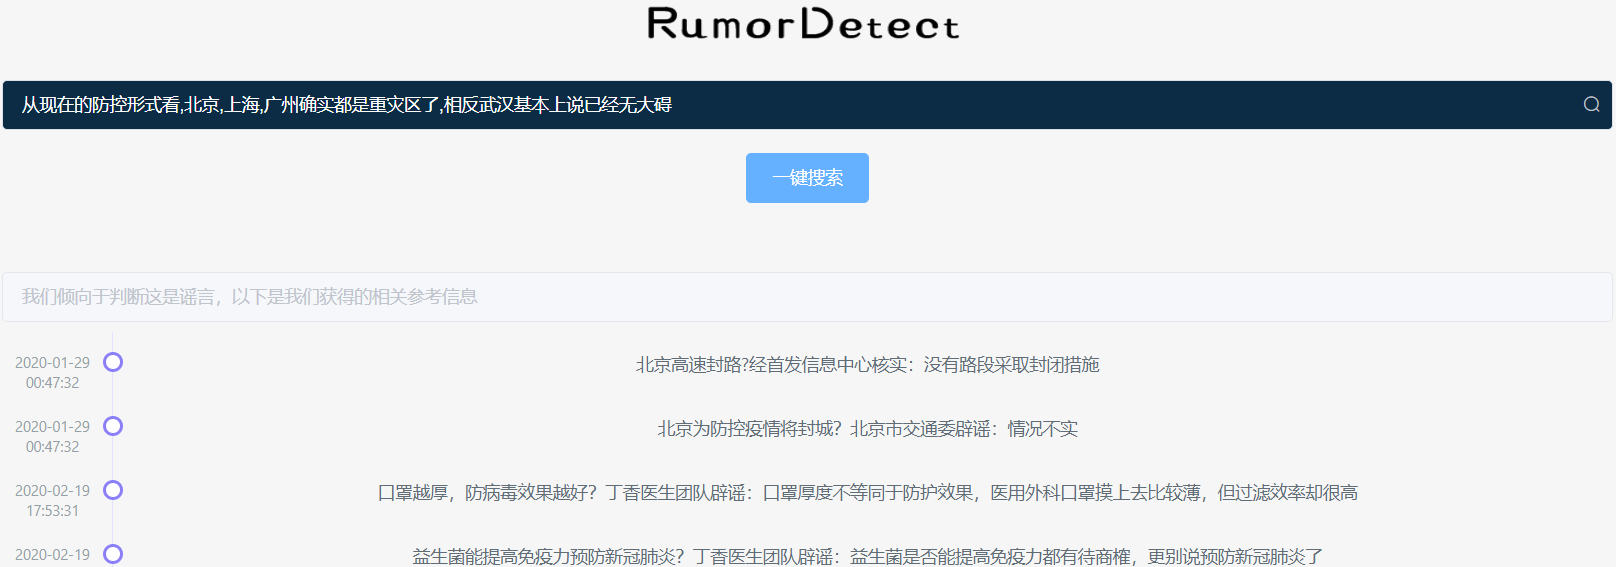
\includegraphics[width=0.8\textwidth]{pic0.png}
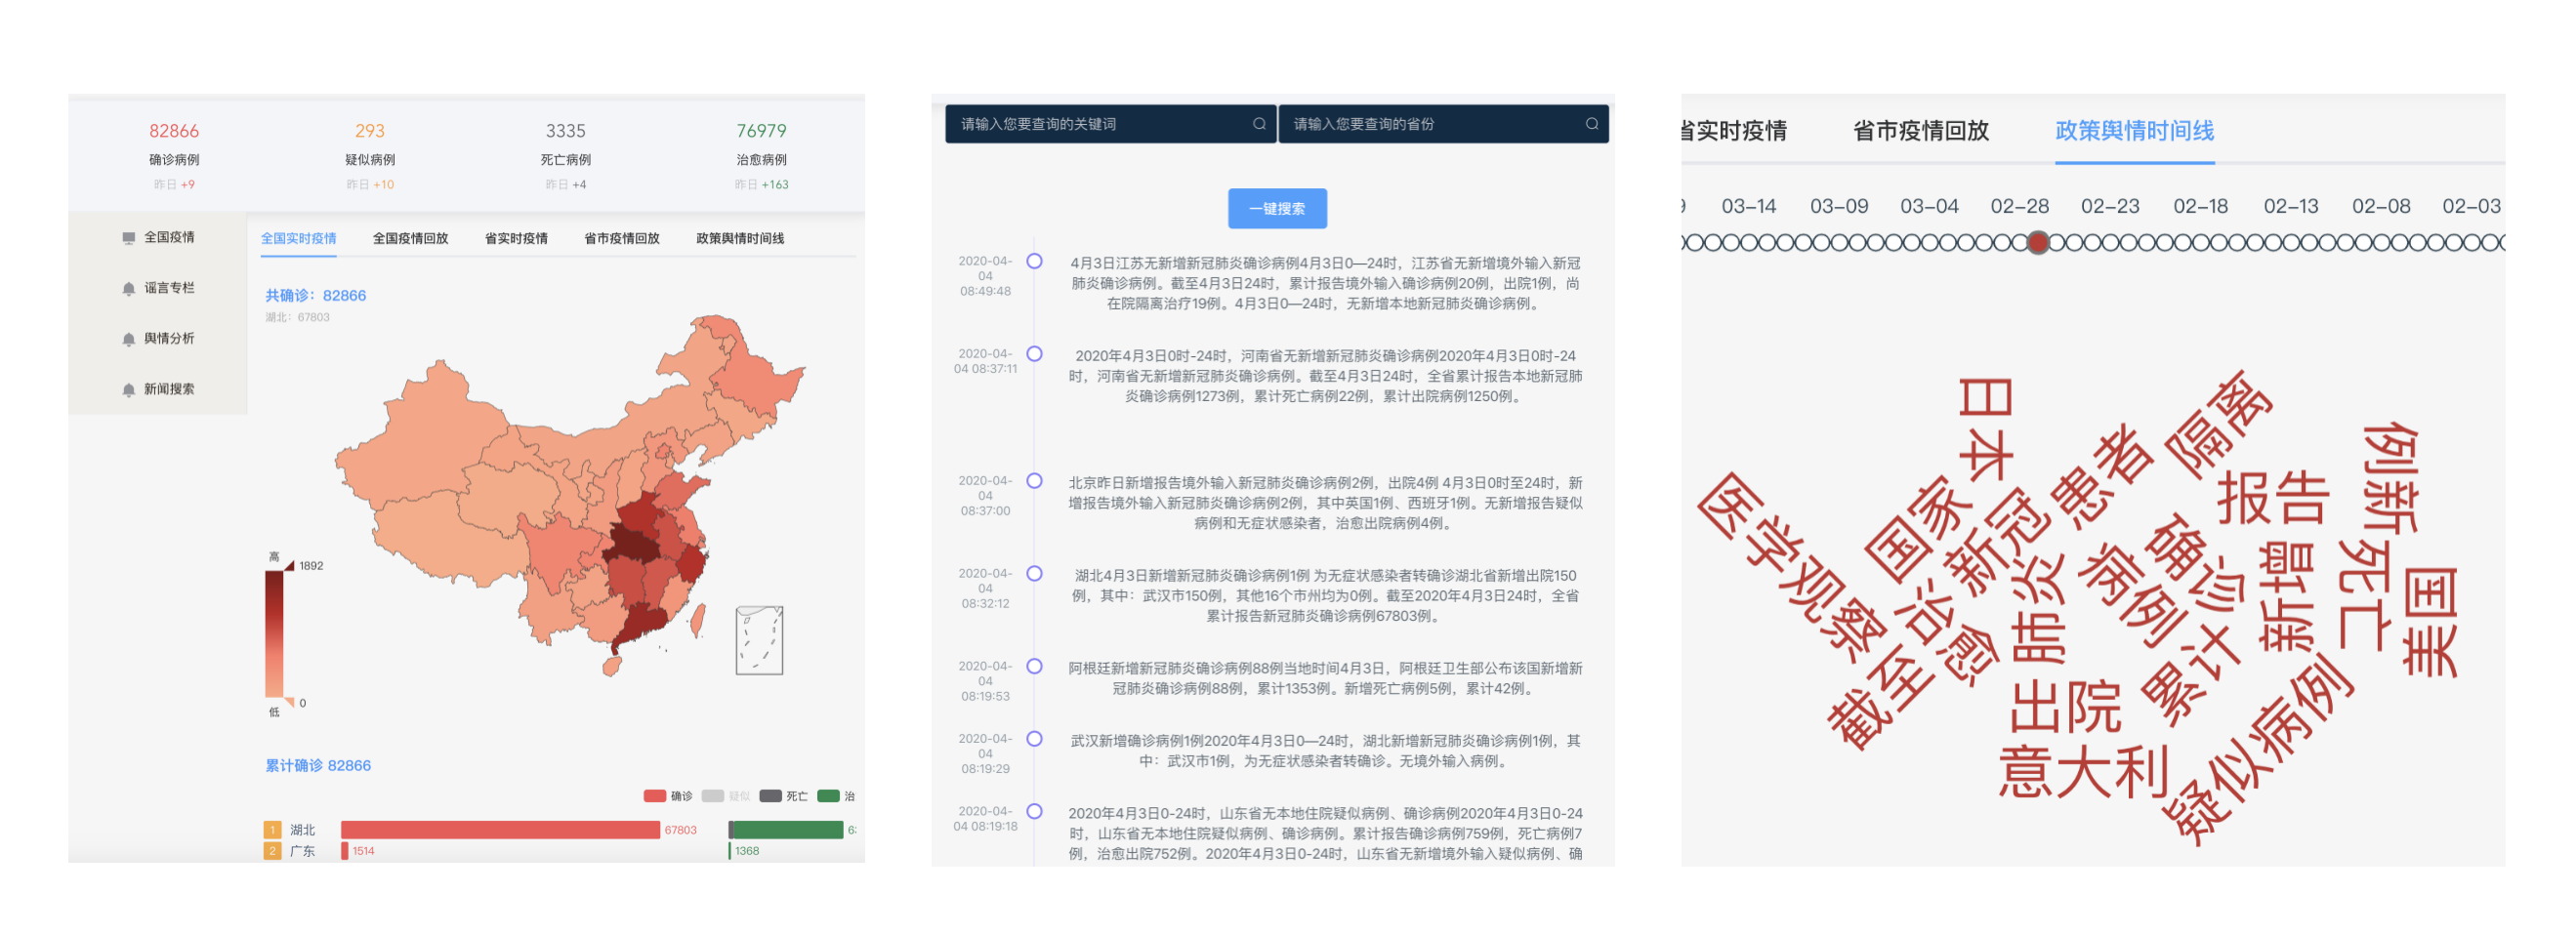
\includegraphics[width=0.9\textwidth]{pic1.png}
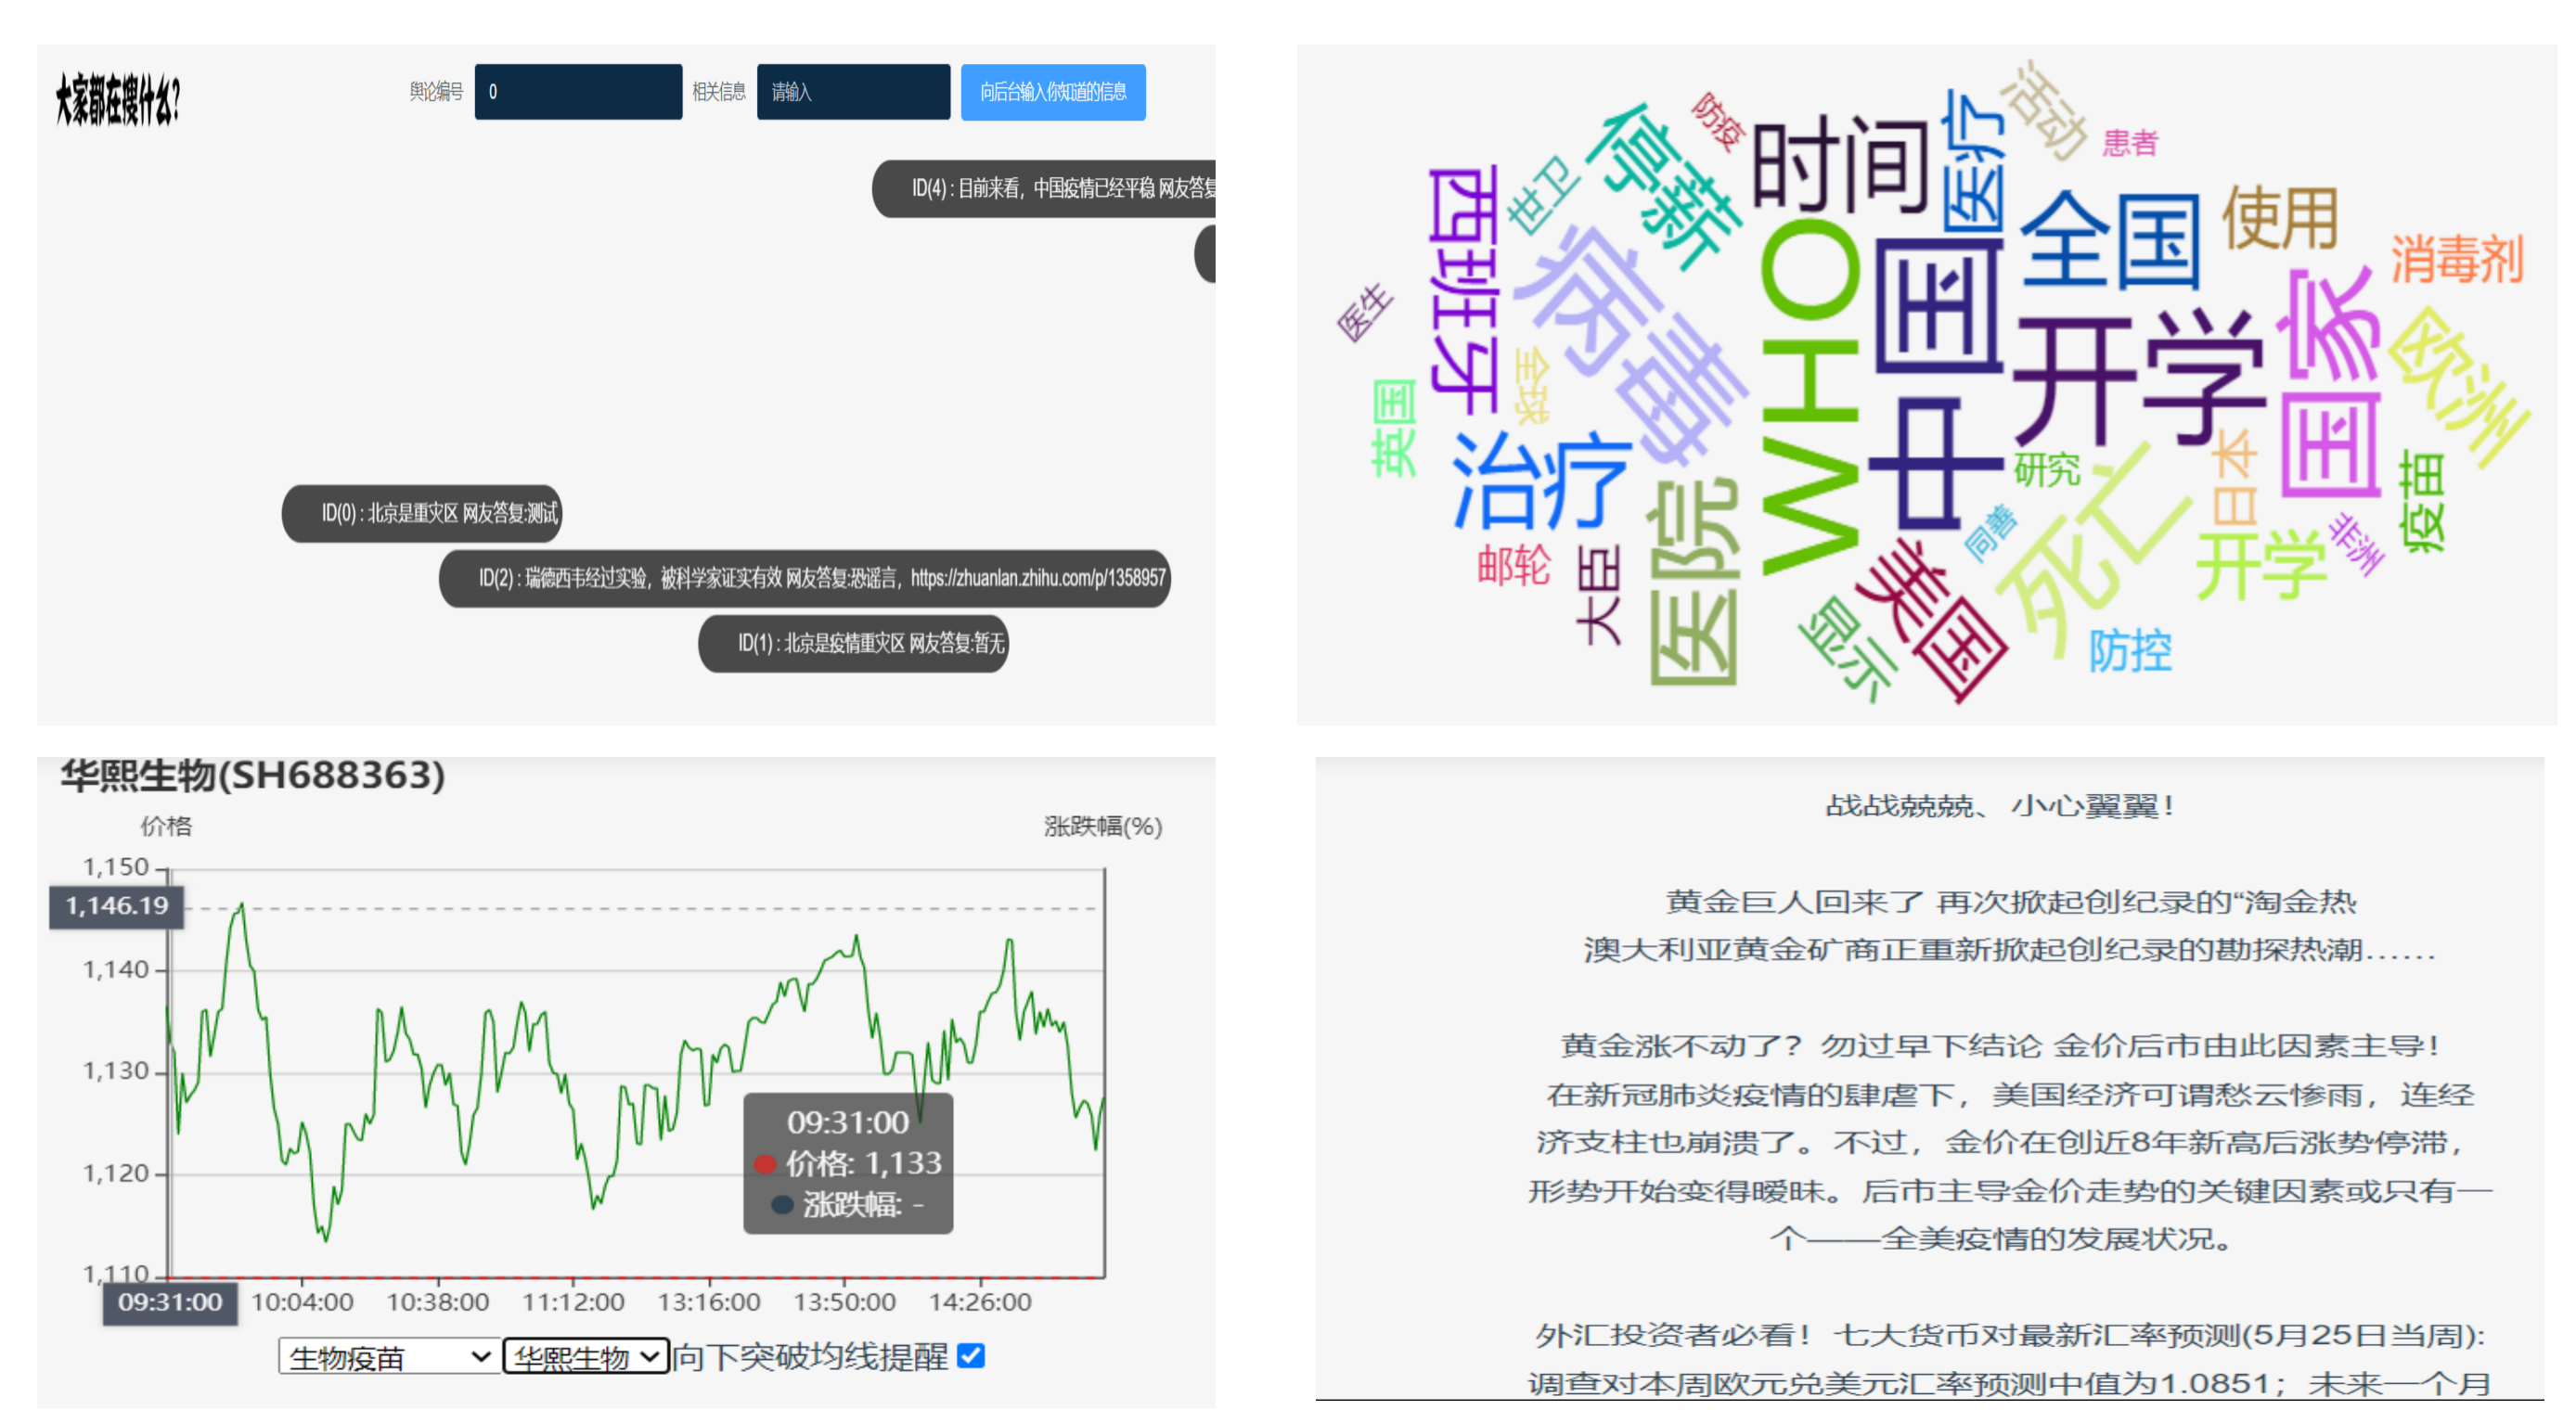
\includegraphics[width=0.9\textwidth]{pic2.png}
\end{figure}

\section{项目特点}
\begin{itemize}
	\item{\textbf{疫情时序数据的维护与展示}\\
	目前主流信息平台微博客户端、新闻网站等提供的信息主要为即时疫情信息,当用户需要了解疫情舆论发展动态或梳理疫情发展趋势时,这就需要使用长时间记录的时序数据,并且目前这种长期的变化数据并不容易获取。}
	\item{\textbf{互动性的舆论判别以及结合人工智能判别与相关真相/谣言推荐的谣言判断系统}\\
	支付宝等平台给出了一些新闻真伪的数据,但它的吸引力并不如它的可靠度那么高。我们更希望获取实时、实地有关的舆论判别,并通过互动式的舆论判别来知道一些自己关心事项的真实程度,并结合政策动态来作出决策。}
	\item{\textbf{在舆论发展序列中提取群众关注热点变化}}\\
	通过对各大平台上发布的新闻、评论数据进行收集,分析群众关注热点在时序上的变化,展示舆论热点随时间上的迁移。
	\item{\textbf{无交易逻辑的轻量市场动态查询}}\\
	我们通过交易平台提供的API,收集疫情题材相关板块个股的市场数据,进行实时更新,且能通过一定的逻辑在个股的一些特殊动态下对用户进行提醒。

\end{itemize}

\section{用户群体}
\begin{itemize}
	\item{希望获得“热搜”以外长期信息的用户。}
	\item{获取信息来源较少、受“浙江十万只鸭派往巴基斯坦治蝗”、“双黄连口服液可抑制新型冠状病毒”等即时热搜影响较大的用户。}
	\item{对地区(不仅限当地)信息、政策更关心的用户。}
	\item{希望利用疫情发展、群众舆论与关注点的用户}
	\item{不了解疫情与市场个股关联、希望得到实时数据反馈的用户(带有交易逻辑的产品有时会有数据滞后、卡顿现象,如中国银行贵金属交易)}
\end{itemize}

\section{项目结构}
\begin{figure}[H]
\centering
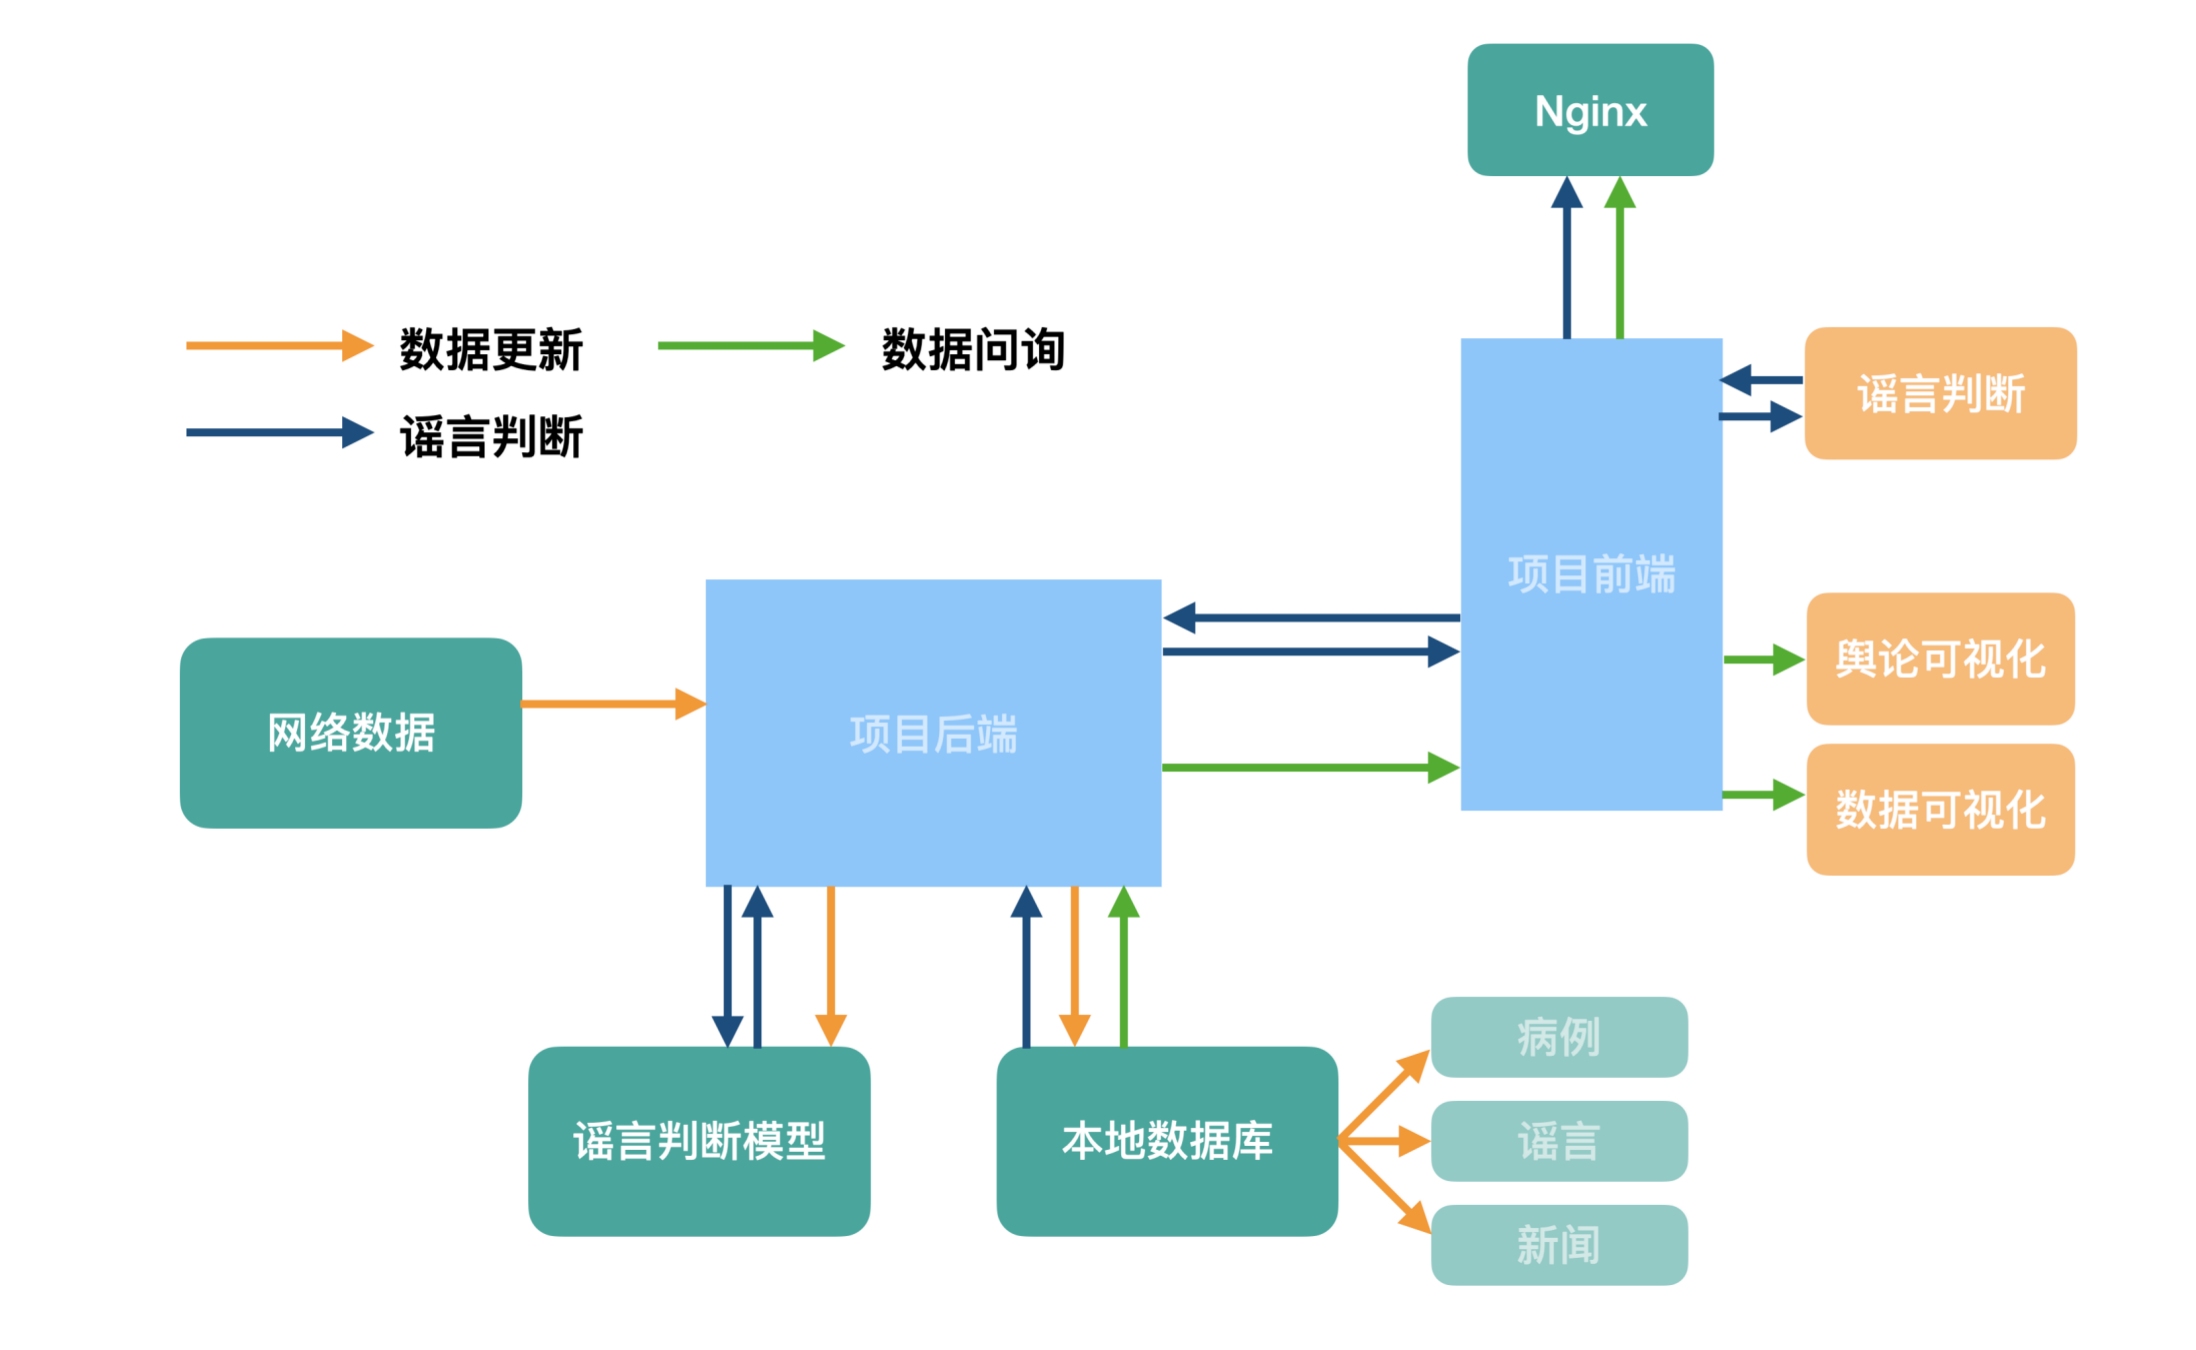
\includegraphics[width=0.8\textwidth]{pic3.png}
\end{figure}

\section{项目关键技术}
\subsection{谣言判断}
\begin{itemize}
	\item{词粒度语义信息提取}
	\item{多头注意力+卷积轻量级模型挂载服务}
	\item{相关谣言辅助识别}
\end{itemize}

\subsection{舆论热点迁移}

\begin{itemize}
	\item{LDA主题模型提取舆论中的关注热点}
	\item{对指定时间粒度上的舆论进行综合分析以及话题提取}
	\item{对话题的“生命周期”、“生长趋势”以及“活跃程度”进行分析}
	\item{对各个热点或话题的交替浮现进行分析与展示}
\end{itemize}


\section{后端接口体系}

目前后端的接口体系已经比较完善,并与前端充分解耦合,可供独立调用,接口可以详细提供我们所收集与分析的数据,供其他有需要的用户自定义使用。

目前拥有成熟调用方法和约定的接口有:
\begin{itemize}
	\item{\textbf{route('/getDataSummary')}} 提供后端数据收集情况概览 
	\item{\textbf{route('/getTimeData')}} 根据时间参数提供全国当天的疫情发展数据
	\item{\textbf{route('/getDataPos')}} 根据地区参数提供该地区的疫情历史发展数据
	\item{\textbf{route('/getNewsData')}} 根据地区和时间参数获取某个地区某个时刻的新闻列表
	\item{\textbf{route('/getRumorData')}} 根据内容类型参数提供该类型的谣言数据
	\item{\textbf{route('/getMap')}} 提供疫情分布的地图数据
	\item{\textbf{route('/getTopic')}} 提供舆论热点话题及变化
	\item{\textbf{route('/getInfoUser')}} 提供用户评价的热点信息
	\item{\textbf{route('/testRumor')}} 预测舆论正确性并提供有关信息
\end{itemize}


\section{项目运行记录}

\subsection{后端的日志}
\subsubsection{站点访问日志}
由于整个后端是使用Flask包装而成的,因此对于后端站点访问的日志是十分重要的。我们在日志中记录了每一次访问的来源、时间、接口和结果等信息,下图为部分记录。

\begin{figure}[H]
\centering
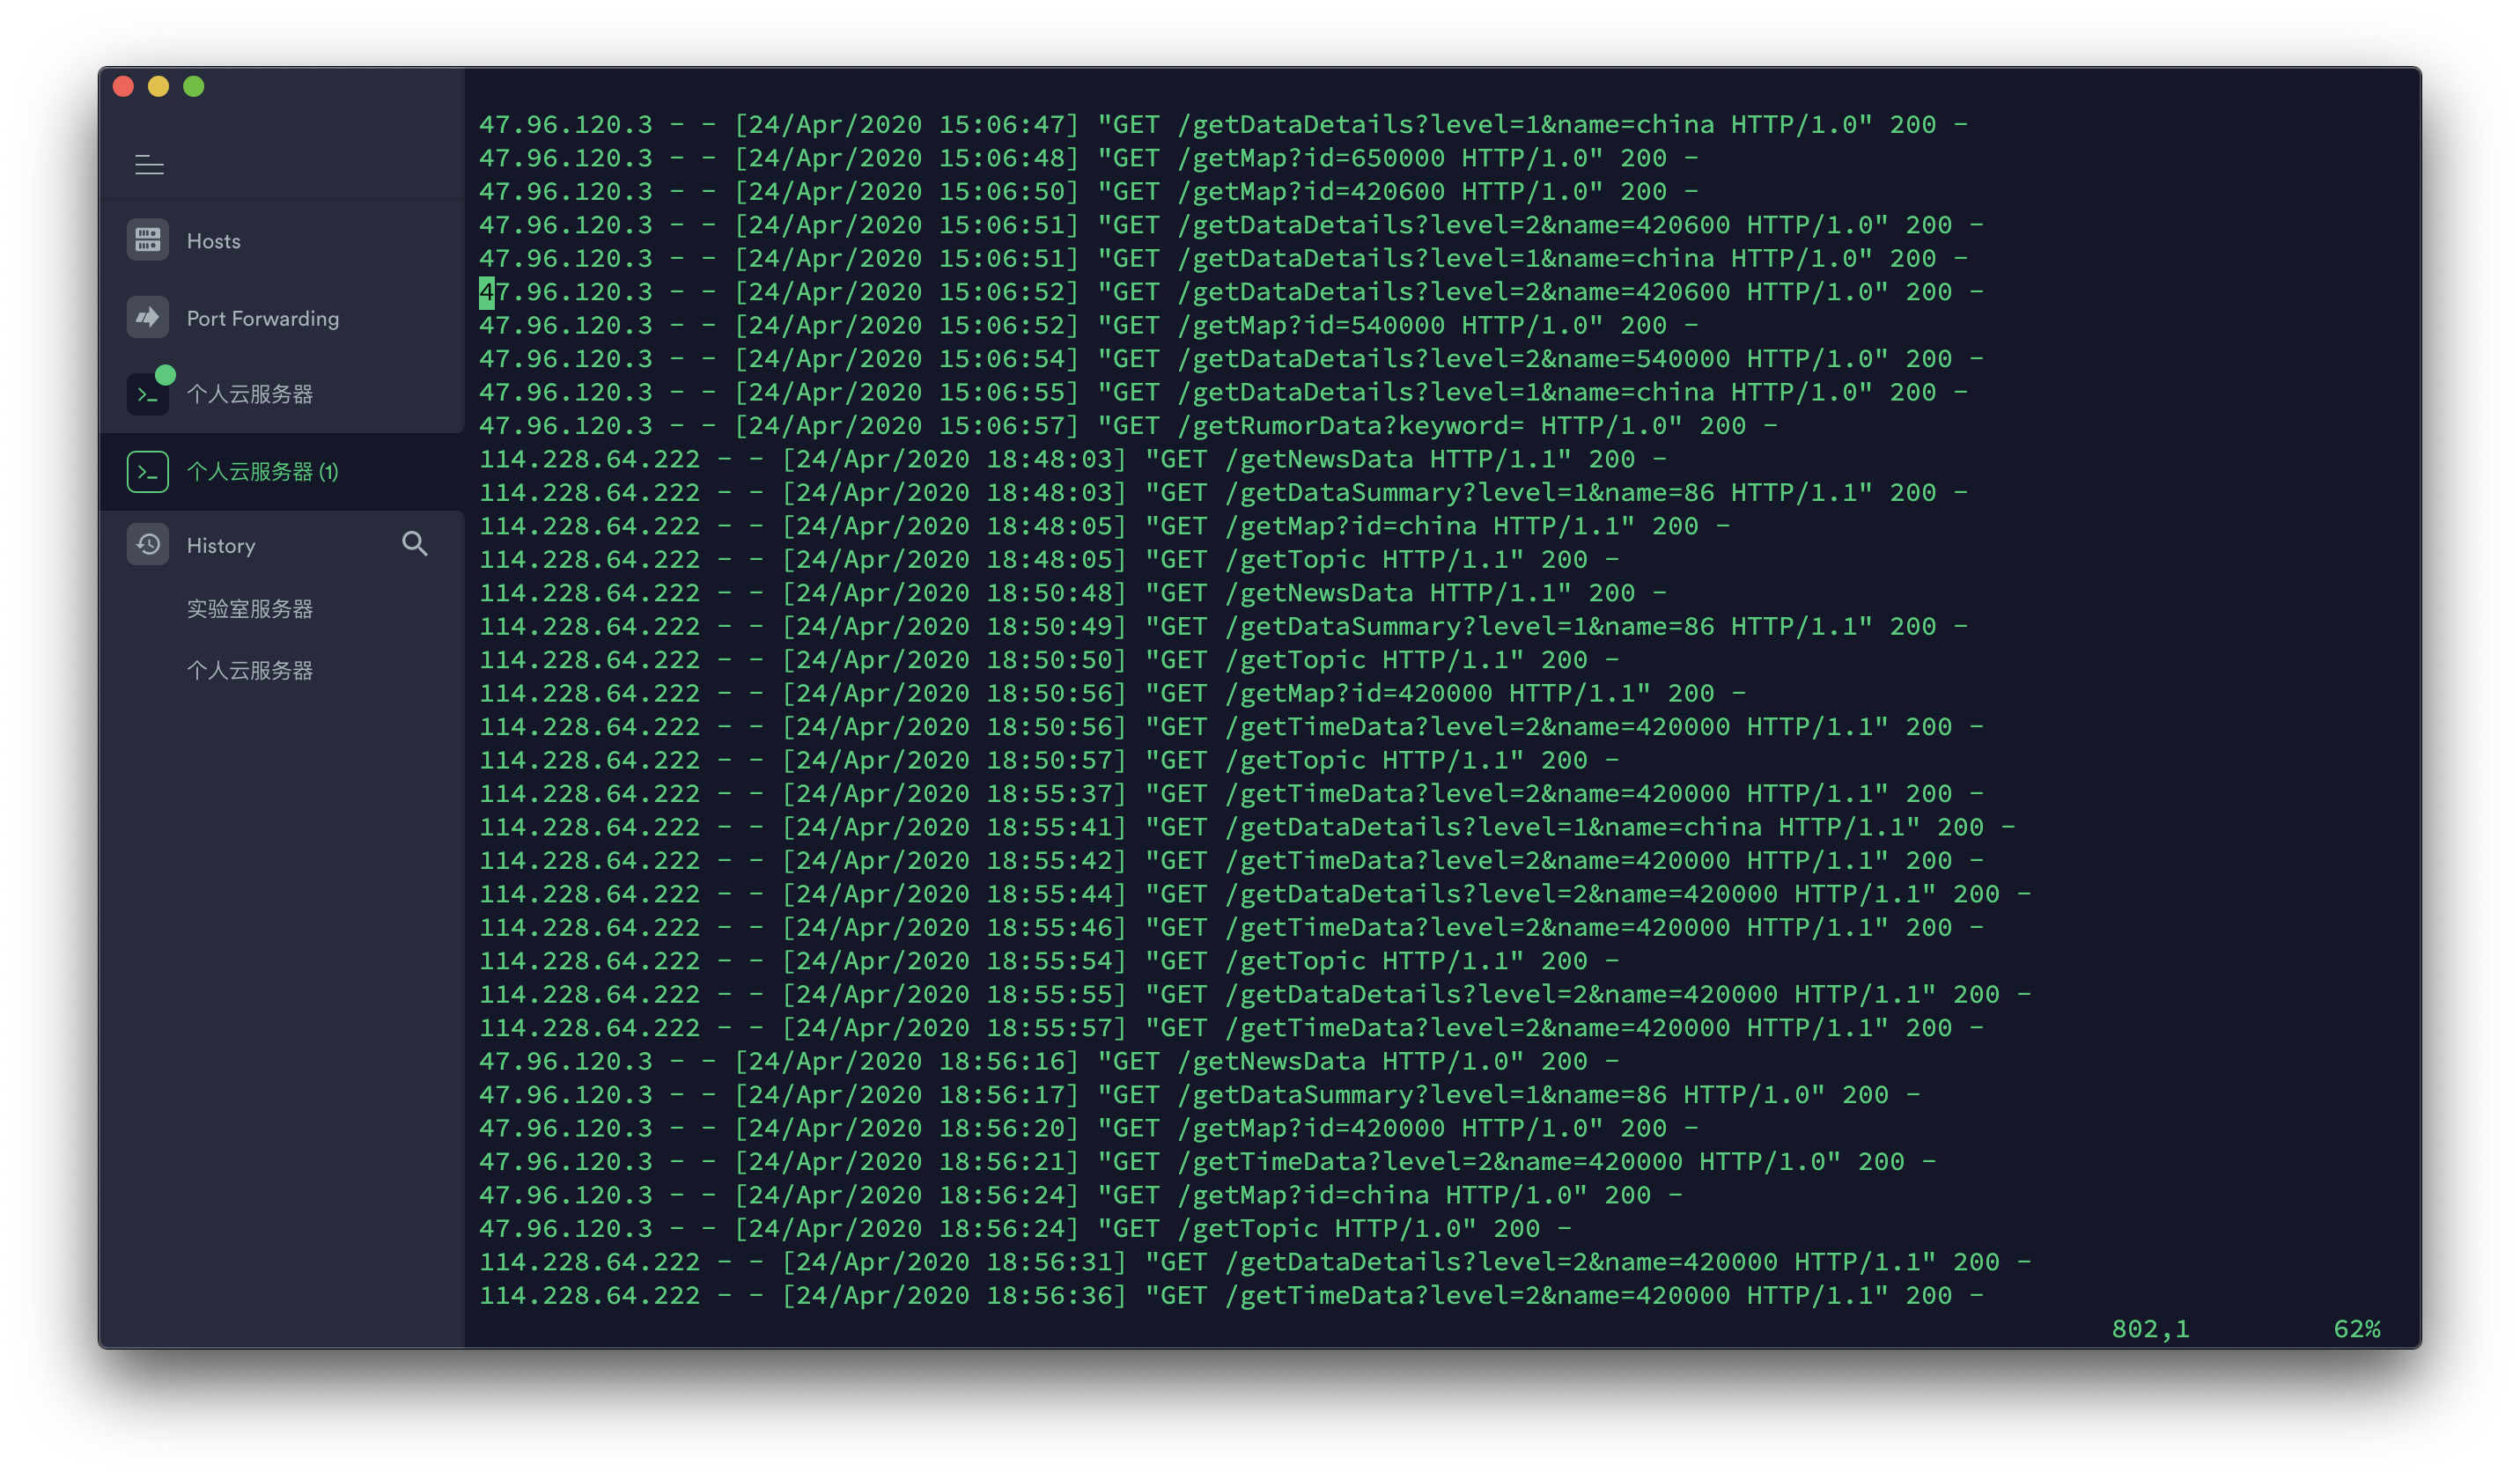
\includegraphics[width=0.8\textwidth]{pic4.png}
\end{figure}

通过站点访问日志我们可以清楚地了解到后端的整体运行情况,并且可以从日志中发现我们项目中的一些问题。例如之前站点访问日志出现了如下条目:

\begin{figure}[H]
\centering
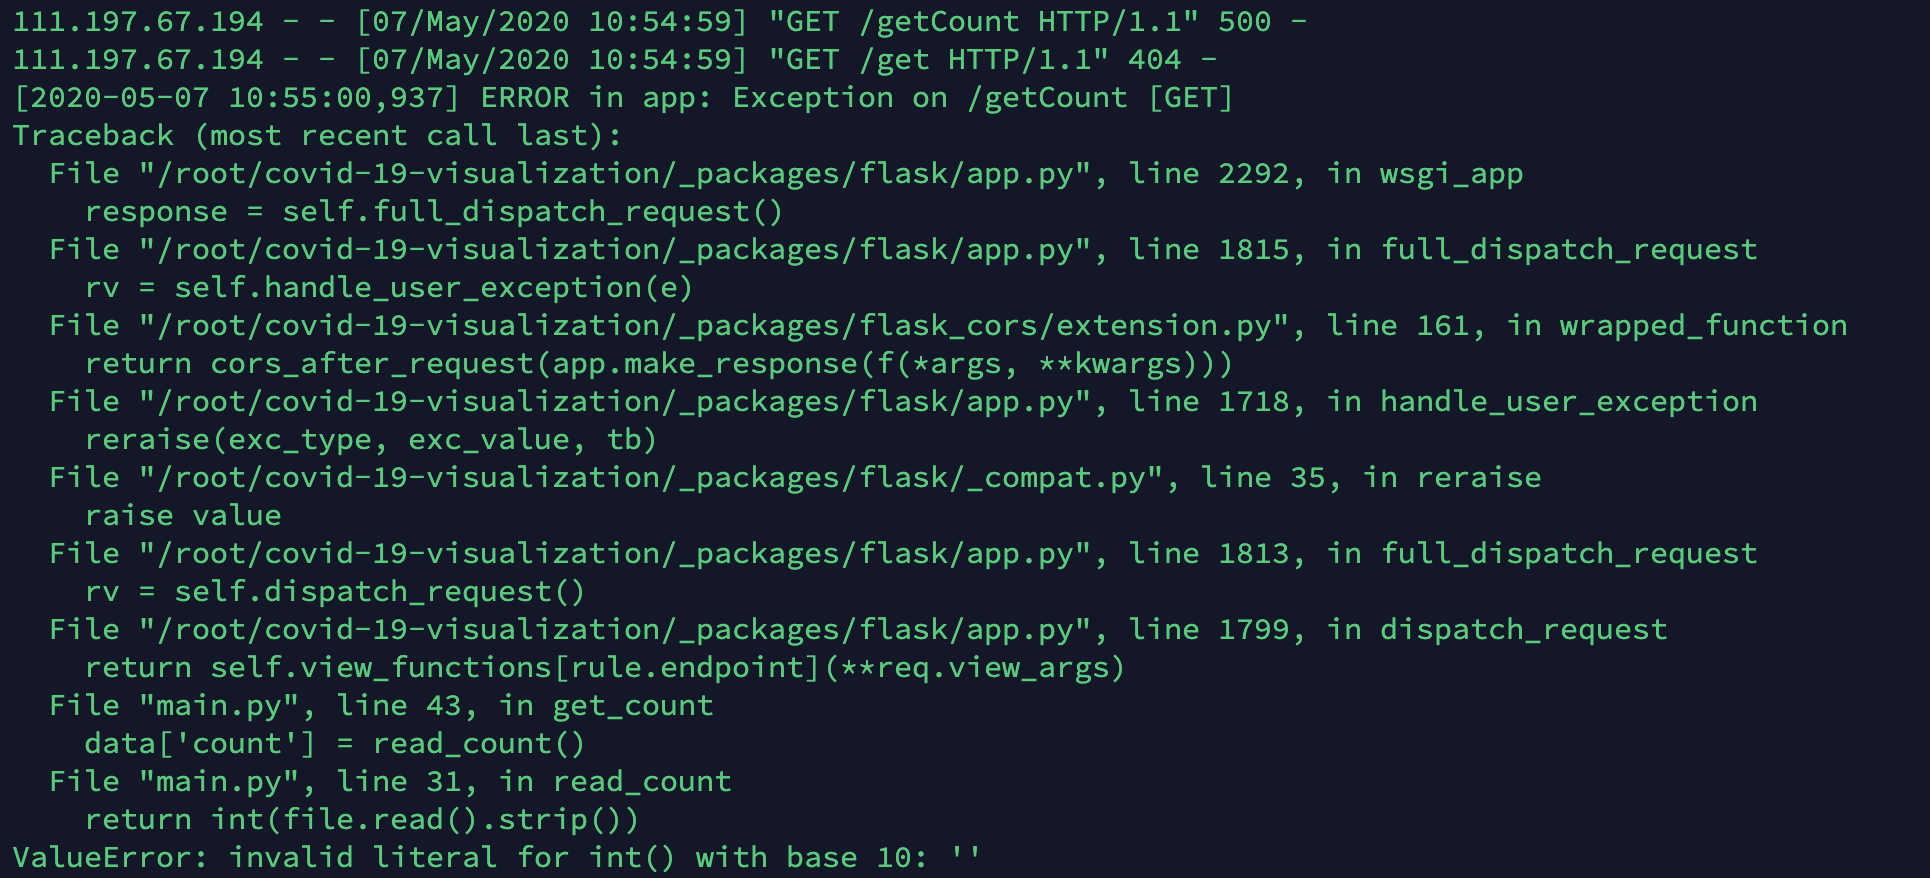
\includegraphics[width=0.8\textwidth]{pic5.png}
\end{figure}

出现该问题是因为某些记录文件被误删除而导致了无法读取数据。发现问题后,我们马上对代码进行修缮,解决了这个问题。

通过站点访问日志,我们可以从整体上了解后端的健康情况,及时发现站点中存在的一些“边界”问题。

\subsubsection{数据访问与更新日志}
后端的重点在于数据的维护,因此数据访问与更新的日志是十分重要的。我们在数据访问与更新日志中记录了每一次向后端申请数据的时间、内容和结果,同时也记录了每一次后端向网络请求数据更新的结果与得到更新数据后数据库更新的结果。下图为部分记录。

\begin{figure}[H]
\centering
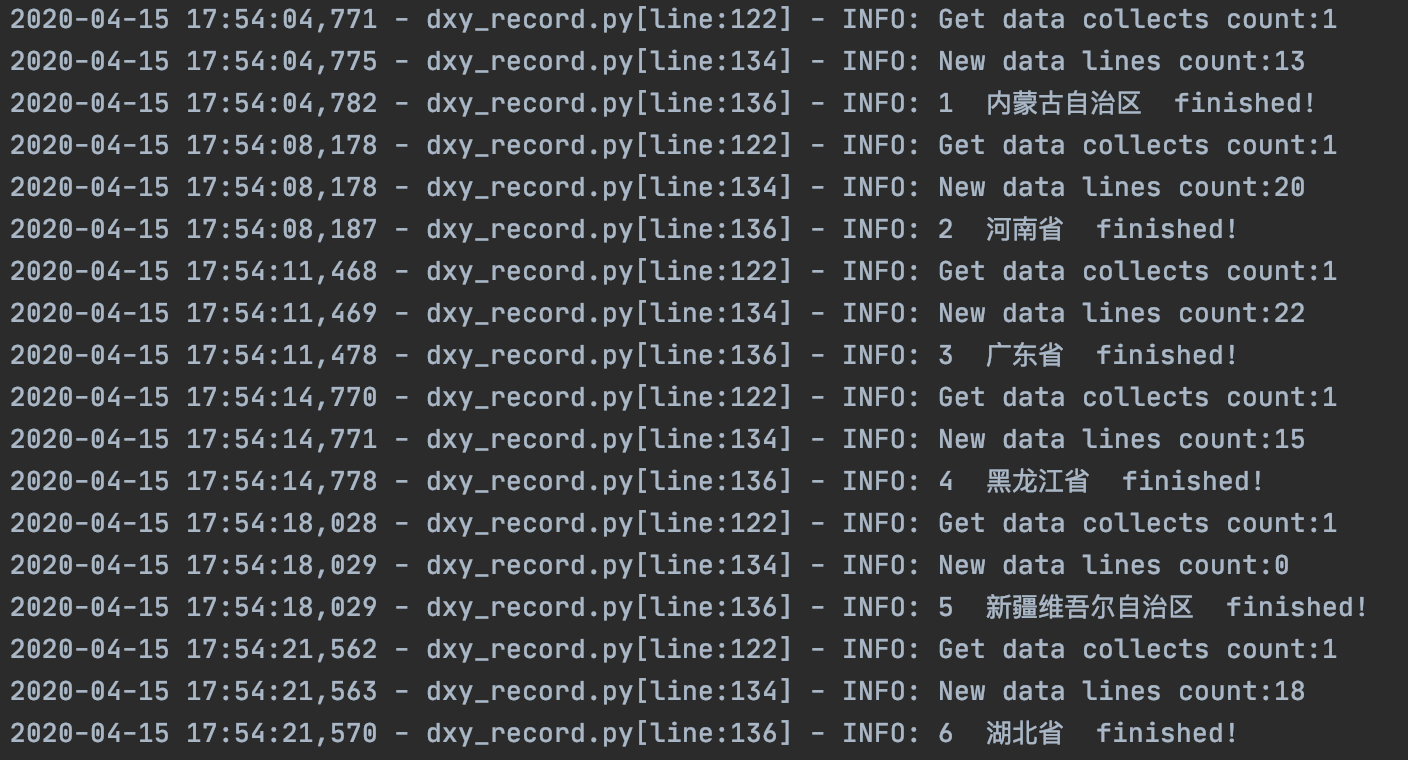
\includegraphics[width=0.8\textwidth]{pic6.png}
\end{figure}

为了更好的了解数据访问与更新情况,我们将日志设置了三个等级:“debug”、“information”和“wrong”。

Debug等级是我们在编写代码测试时使用的一种极其详细的日志等级,因为日志十分冗余,在项目上线运行时一般不需要查看该等级的日志。

Information等级是项目运行时记录访问与更新情况用的较多的一个等级,在该等级中,我们会详细记录每一次的后端操作的信息,例如上图就是数据更新操作的Information等级日志。

Wrong等级日志是项目运行时记录我们认为不应该出现的情况,例如“向网络请求数据更新得到空条目”,在中期报告不久后的时间,我们发现虽然后端数据自动更新的程序在运行着,但是数据库内数据停滞更新了,通过查看日志我们发现,时原来使用的某个API接口停止服务了,得到该信息后,我们迅速修改了更新的相关流程,将后端数据更新。


\subsubsection{日志的部署与记录方式}
项目后端的重点是数据的维护,面对庞大的维护信息,日志记录是一个强大的助手,因此我们十分重视日志记录,在项目开始时就部署了以上两部分日志。

为了方便及时阅读,后端的日志是以纯文本的方式记录的,不同方面,不同等级的日志分别处于不同的文件中,我会在本机运行Python程序定时将远程服务器的日志文件拷贝到本机进行异常检查,以便及时发现问题,修复问题。


\subsubsection{日志量}

站点访问日志根据我们站点的访问次数而定,每有一次访问时会增加一条记录,因此日志数量并不固定。

由于后端的数据自动更新程序每30分钟会网络请求数据更新,因此数据访问与更新日志中的Information等级日志日志量较大,达到约每天6000行左右,其中记录数据更新的日志占90\%左右。

数据访问与更新日志中的Wrong等级日志主要记录后端中的异常情况,现在我们的项目已经稳定的运行,因此日志量较小,近一周平均每天约7.3行。

数据访问与更新日志中的Debug等级日志主要为调试代码使用,因此不在此讨论日志量。

\subsection{前端的日志}
前端通过nginx实现持续挂载,在初步实现挂载时开始进行日志记录,对访问信息日志$access.log$和错误信息日志$error.log$进行维护,均保存在nginx服务器的日志保存目录中。
\subsubsection{访问日志}
访问日志主要包括如下具体内容:(1) 客户端(具体用户)IP地址,例如一开始主要是“222.185.220.44”,这是本组前端维护者的IP,之后地址逐渐多样化,代表开始在用户中得到推广;(2) 访问时间;(3) 请求的URL地址、请求状态、请求页面大小; (4) 请求页面大小; (5) 来源页面; (6)浏览器信息
我们目前通过简单的离线执行的(非实时运行)代码,从访问日志中作两类信息的利用:统计用户来源;数据传输量。数据传输量是为了下一步进行性能优化作参考。
下图为部分记录
\begin{figure}[H]
\centering
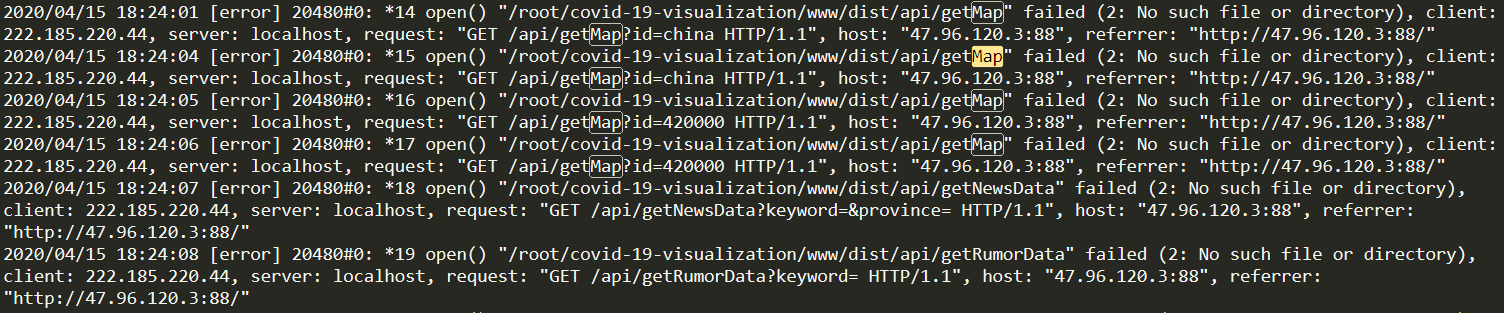
\includegraphics[width=0.8\textwidth]{access.png}
\end{figure}
\subsubsection{错误日志}
错误日志重点内容在于错误信息,主要结合其中的请求内容、错误提示观察其中的错误类型,目前遇到的问题主要为两类:重新build导致暂时的文件缺失、后端调整导致的访问失败。
下图为部分记录
\begin{figure}[H]
\centering
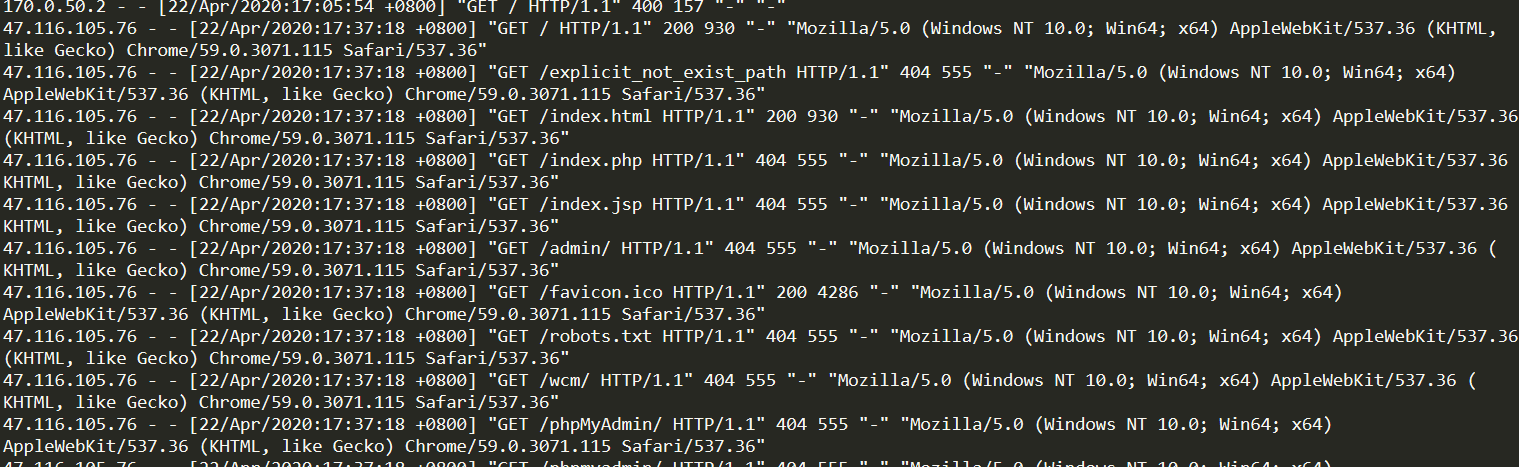
\includegraphics[width=0.8\textwidth]{error.png}
\end{figure}
\subsubsection{日志的部署与记录方式}
前端通过nginx实现持续挂载,在初步实现挂载时开始进行日志记录,对访问信息日志access.log和错误信息日志error.log进行维护,均保存在nginx服务器的日志保存目录中
\subsubsection{日志量}
目前错误日志大约共一百余条,均为调整产生;访问日志日均30条。我们参考了已有的实现方式,进行日志切割,按日期进行存放。


\section{项目负载均衡性能}

\subsection{我们的负载均衡方法}
我们采用fair策略,根据页面大小、加载时间长短智能的进行负载均衡。该方法在初始的nginx中并没有支持,需要我们手工添加附加包、修改原先的结构体来实现新算法。

我们原计划在原服务器中建立四个服务,提供四个端口,但为了提高系统的可用性,并且接近真实的负载均衡、进行实验,我们后续加入了一台腾讯云单核服务器,与原计划效果进行对比。



\subsection{负载均衡实现检验}
我们分别核验后端多个服务的访问日志、停止一部分服务来检验负载均衡的效果。
我们暂时中断175.24.30.4上的所有服务,此时我们的网页仍能正常使用,且因为剩下的服务提供数据更快,延迟更小了。而观察所有后端日志,可以发现不同服务的访问日志行数大致相等。

\subsection{负载测试}
我们使用JMETER的取样器、监听器,实现不同的请求,查看单位时间延迟和吞吐量。
我们测试20个线程,Rame-Up Period(启动时间,即所有线程全部启动花费时间(s))设为10秒。我们需要大概十分钟到十五分钟完成一次一般的负载测试、获得稳定的结果。

我们可以生成数字和图形形式的报表。
\begin{figure}[H]
\centering
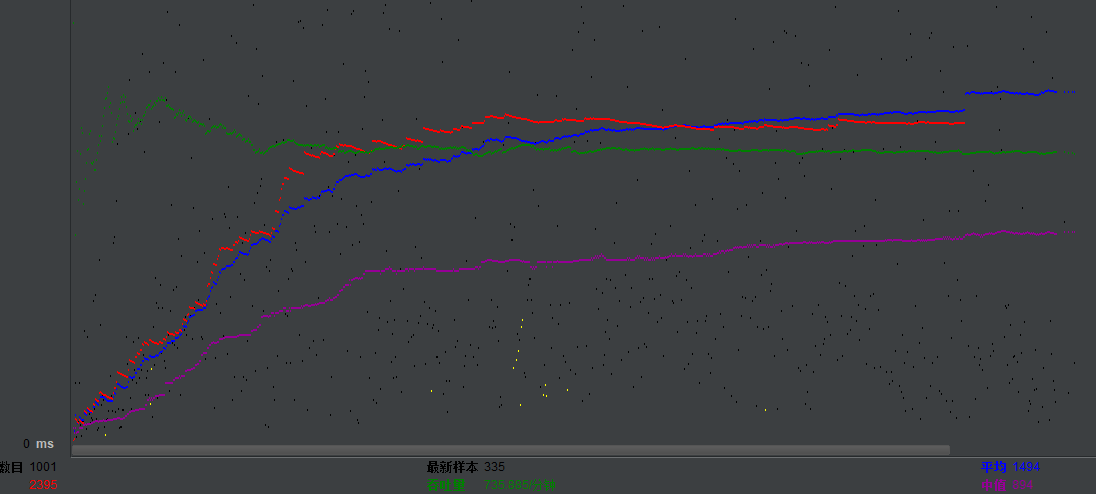
\includegraphics[width=0.85\textwidth]{graph.png}
\end{figure}
\begin{figure}[H]
\centering
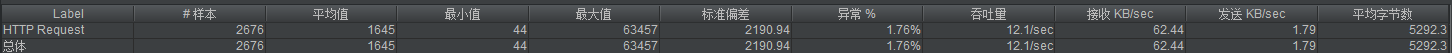
\includegraphics[width=0.85\textwidth]{figure.png}
\end{figure}
\subsubsection{单场景测试}
我们暂时只加入全国信息查询,获得结果:平均延迟为1811ms,吞吐量为10.4/sec。
\subsubsection{多场景测试}
我们同时加入了新闻查询、谣言查询和全国疫情信息查询三个http请求配置元件。在单线程中,我们发现其latency具有显著差别,全国疫情信息延迟最高,是另两个的若干倍。多场景测试比较贴近实际情况,用户的具体请求有差别。

在我们Nginx使用朴素轮询策略时,我们得到的平均延迟为1655ms,吞吐量为11.9/sec,我们使用加载时间适应策略时,得到的平均延迟为1569ms,吞吐量为12.1/sec。

为何表现基本相近?原因在于当我们使用相同的服务器、不同的服务器有同样的工作环境,此时并不会产生不同服务之间延迟的明显差异,所以两种方法不会有太大差别。

后续我们引入新的服务器,我们发现引入这反而使得整体速度变慢,通过ping、查看JMeter的报告,我们发现是该服务器上挂载服务的通信时间过长所致。在这种情况下,我们后续将其作为备用服务器,提高整体系统的可用性。

不过这种情况下我们也测试出了fair策略和朴素轮询策略的优劣。我们在朴素轮询策略下,获得的平均延迟为4075ms,吞吐量为4.2/sec;而fair策略下,我们获得的平均延迟为2930ms,吞吐量为5.3/sec。说明fair策略确实做到了考量页面和加载时间来分配负载。

\section{项目开发经历}

\begin{figure}[H]
\centering
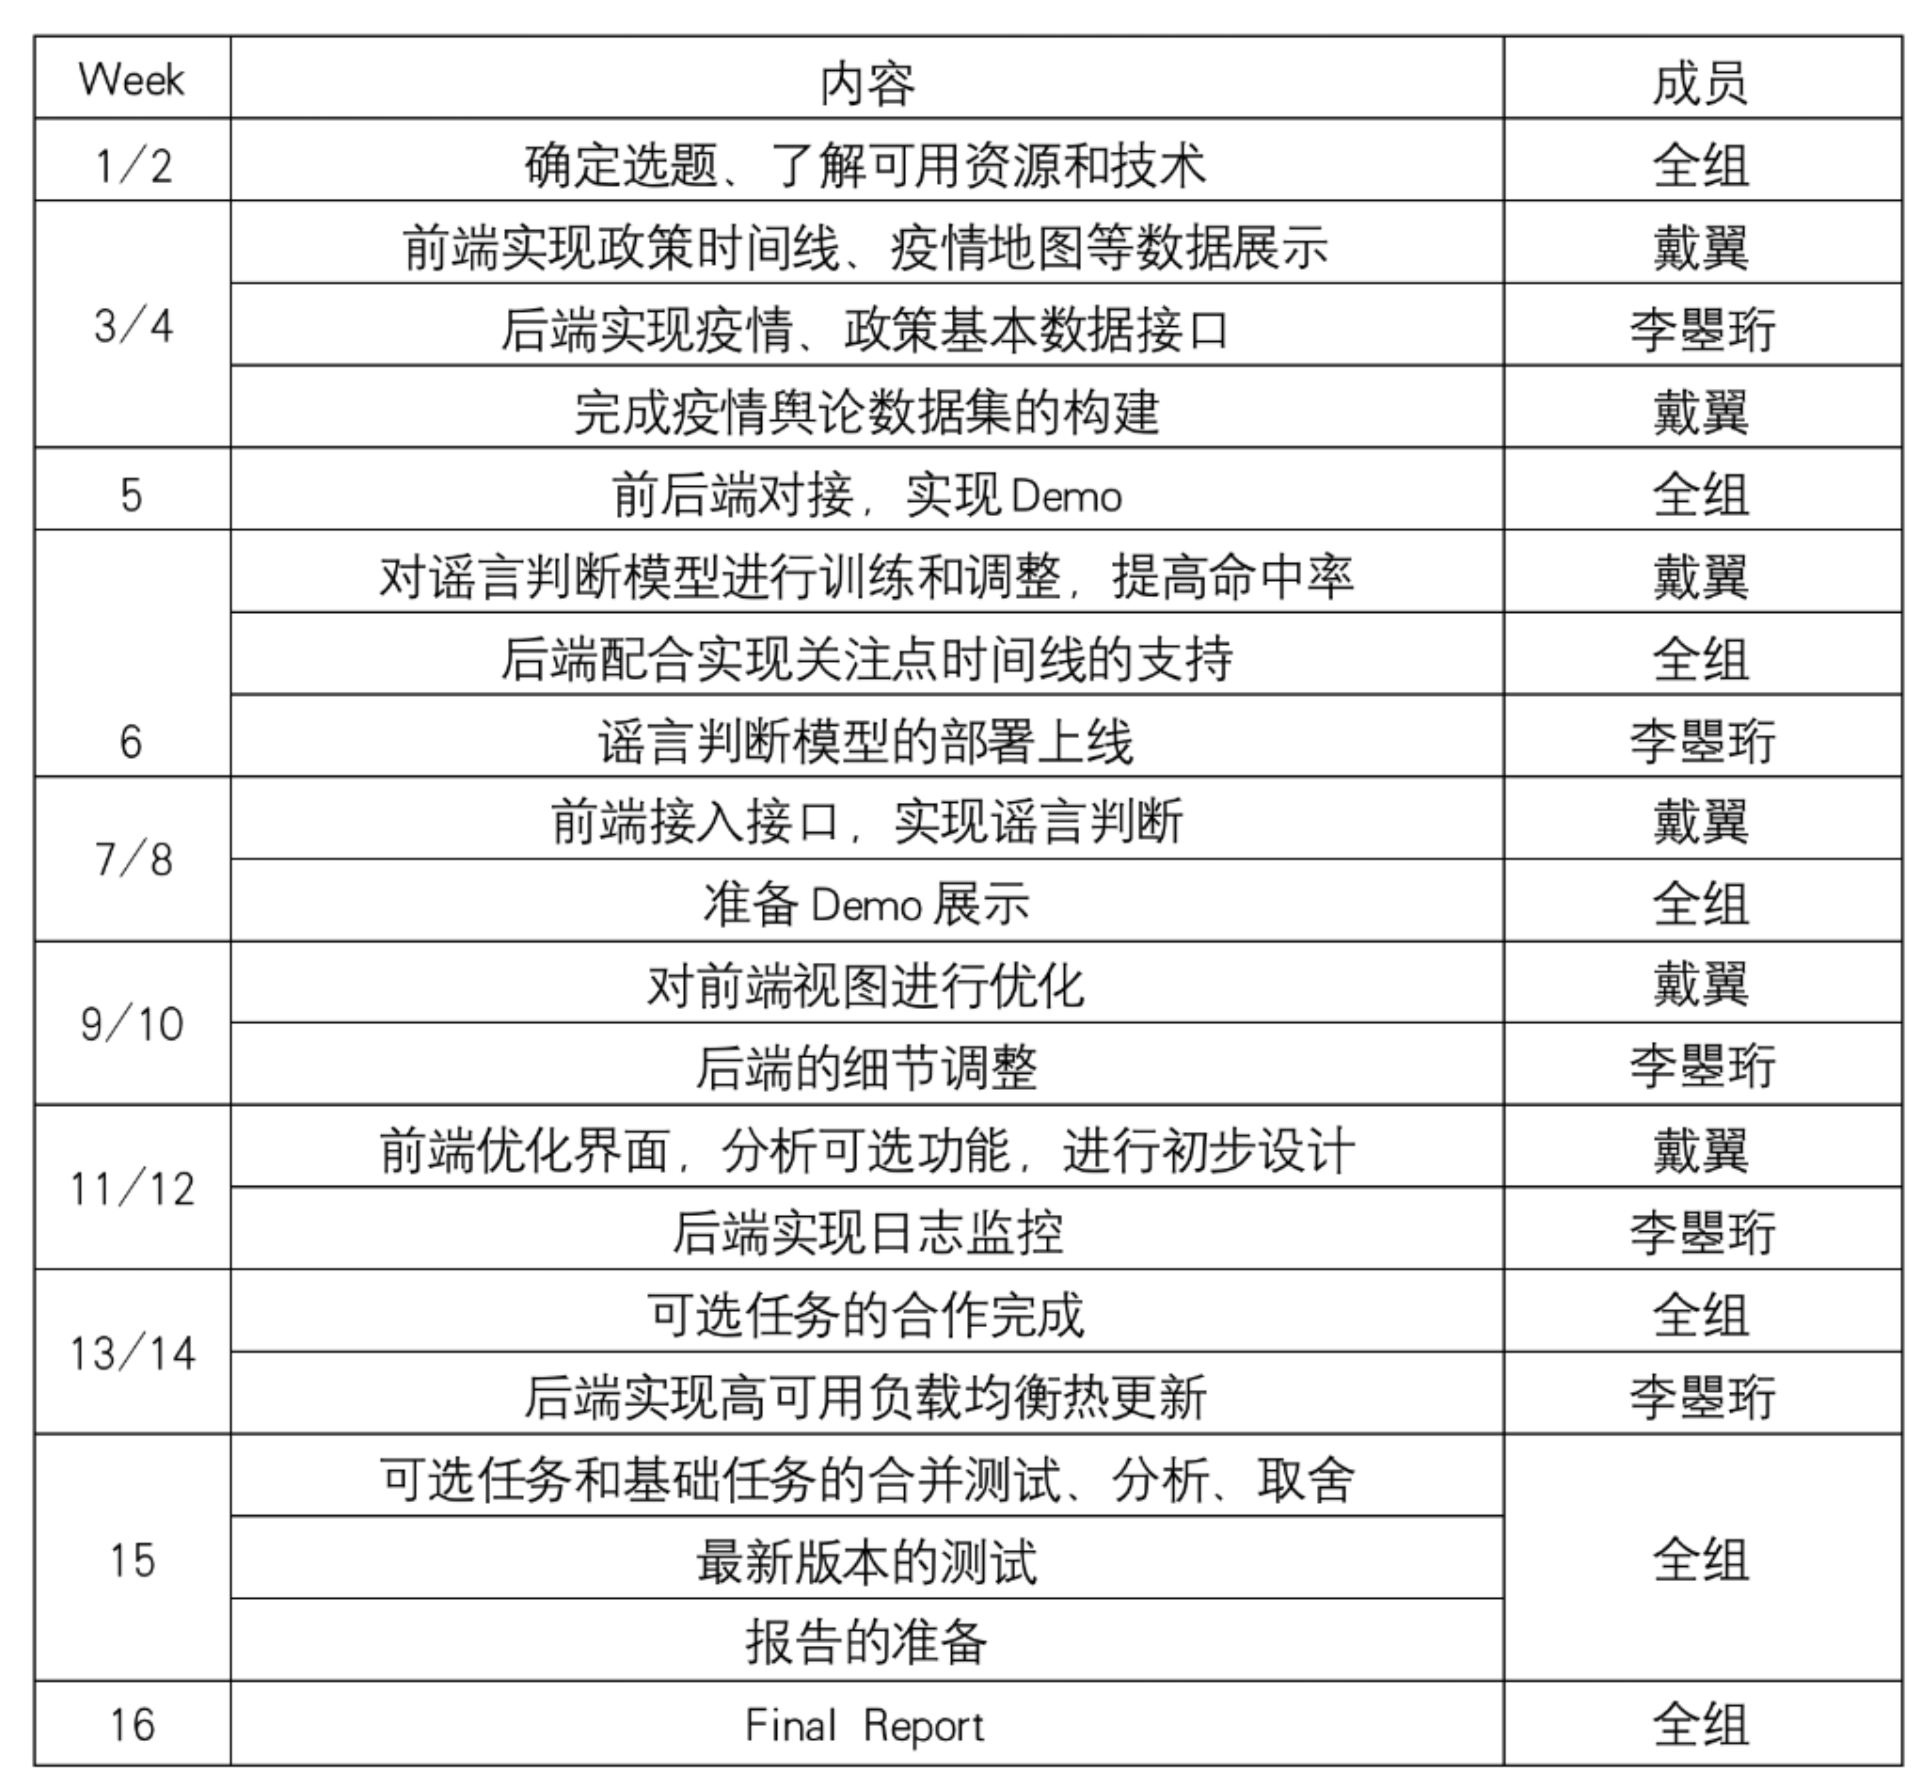
\includegraphics[width=0.85\textwidth]{sche.png}
\end{figure}

我们在项目初期制定了项目开发的计划,并且如期地、有序地、较为顺利地按照计划进行开发。在开发中,我们也遇到并解决了一些较为棘手的问题,有些问题是我们自己发现的,也有一些是老师和同学们提出的,在此感谢大家。


\subsection{舆论数据集收集问题以及解决方案}

在项目开发中期时,我们发现在舆论热点迁移的分析过程中,由于我们获取的新闻数据内容比较单一,导致每个时间粒度下提取出的热点、话题内容比较相似,迁移程度不太明显。对此我们采用的解决办法是多方大量再收集数据,从微博上爬取相关的新闻、用户的评论等信息来丰富我们的数据库。

我们从新浪微博中爬取了人民日报账号下关于新冠病毒的相关新闻约4000条文本,加入了我们的舆论数据库中,使舆论热点部分分析的语料库更加丰富,同时对热点词的抽取算法做了一些改进,过滤掉一些较为频繁但无意义的词汇,例如“新冠”、“病毒”等。

下图为改进的结果,左图为改进前,右图为改进后。

\begin{figure}[H]
\centering

\includegraphics[width=0.4\textwidth]{word-old.png}

\includegraphics[width=0.5\textwidth]{word-new.png}
\end{figure}

\subsection{前端用户体验的改善}

在中期报告中,用户提出了一系列的体验感受和建议,其中最重要的就是信息加载时的空白屏现象。一般前端开发者有“可能触发用户等待行为的操作”的说法,我们将这类切换都加上了过渡动画,并进一步缩短了加载时间。

之前还有用户线下反馈了点击全国地图省区无法直接跳转到目标省份地图的问题,我们也进行了修复。

\begin{figure}[H]
\centering
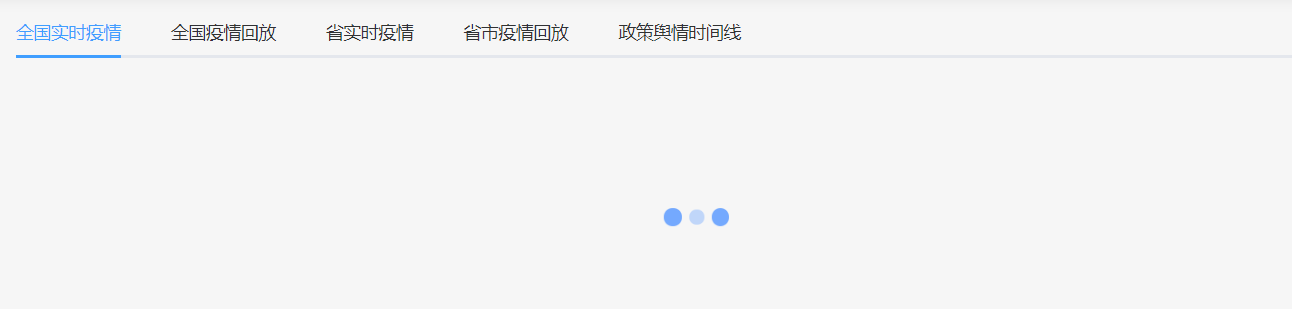
\includegraphics[width=0.8\textwidth]{pic7.png}
\end{figure}

\subsection{前端视图和互动优化}

我们在中期报告中发现JustDropIt组采用的词云展示性更好,我们在之前的词云上加了随机颜色处理,并且加上了云状外框,根据权重关键词体积可以自适应大小等功能。


\begin{figure}[H]
\centering

\includegraphics[width=0.8\textwidth]{word-new.png}
\end{figure}

我们还发现目前的界面互动性不够充分,目前采用弹幕+文本框的方式,也是一个辅助谣言判断的新功能:用户可以看到使用者群体的查询信息、上传和阅览相关的信息更新,实现一个扁平的“社区”。该功能我们正在向同学调研体验。

\begin{figure}[H]
\centering

\includegraphics[width=0.8\textwidth]{pic9.png}
\end{figure}


\section{项目未来发展}

目前项目利用负载均衡技术在两台服务器中平稳运行,由于项目在我们的个人服务器中,我们计划未来将项目进行细致调整和优化后一直运行下去。

我们发现目前在Github社区中并没有类似我们疫情经济模块的工具包或代码片段,我们试图将现有的工作整理,包括股价特殊动态的提醒逻辑,单独打包发布。

由于在域名申请的过程中,我们被告知个人性质的网站是不能展示疫情数据的,因此我们的备案不能通过。没有域名以及有力的宣传手段,这导致我们网站的日均访问量不高,约为每天20次左右。但是我们认为,疫情发展的历史数据、舆论和经济数据对于回顾和分析整个疫情发展过程是十分重要的,因此我们将数据开放给社区使用。后端的接口体系已经比较完善,并与前端充分解耦合,可供独立调用,接口可以详细提供我们所收集与分析的数据,供其他有需要的用户自定义使用。

目前拥有成熟调用方法和约定的接口有:
\begin{itemize}
	\item{\textbf{route('/getDataSummary')}} 提供后端数据收集情况概览 
	\item{\textbf{route('/getTimeData')}} 根据时间参数提供全国当天的疫情发展数据
	\item{\textbf{route('/getDataPos')}} 根据地区参数提供该地区的疫情历史发展数据
	\item{\textbf{route('/getNewsData')}} 根据地区和时间参数获取某个地区某个时刻的新闻列表
	\item{\textbf{route('/getRumorData')}} 根据内容类型参数提供该类型的谣言数据
	\item{\textbf{route('/getMap')}} 提供疫情分布的地图数据
	\item{\textbf{route('/getTopic')}} 提供舆论热点话题及变化
	\item{\textbf{route('/getInfoUser')}} 提供用户评价的热点信息
	\item{\textbf{route('/testRumor')}} 预测舆论正确性并提供有关信息
\end{itemize}


\section{ISOA课程总结}

首先非常感谢老师和助教为我们提供的帮助,使我们能够顺利地开发出一个优秀的项目并成功上线运行。

%%对于整个课程以及所做项目的感想,包括学到了什么新的内容、对于什么技术有了更深的了解、在写代码或是团队合作上有什么心得、以及对于课程内容、授课方式有什么意见和建议。
在这一整个学期中,我们经历了项目设计、开发、部署和优化的全过程,在过程中我们接触了新的领域,学习了新的技术和内容,同时也巩固了已经掌握的技能。


在初期项目设计的时候,我们在选题过程中花费了较长的时间,因为选题方向直接确定了我们这一学期的工作内容、工作重点和难度。由于课程将选题限定在两个大方向内,我们先搜索了相关领域选题的已有工作和现有数据集完备情况,然后经过讨论后,我们决定做疫情舆论相关内容。原因是社会上对于疫情的病例数据已经有较为完全的数据发布以及分析情况,但是我们发现对于舆论方面缺少相关的分析型网站。在疫情中舆论的话题导向相关内容可以充分的反映出群众心态、关注点的变化,这对于分析疫情对人民影响情况有极大的帮助,具有较大的利用价值。另外对于疫情舆论数据我们可以在各大网站进行爬取获得,数据集获取并不困难。总体而言,这个项目选题可实施性和实用性较强,因此我们选择了这个题目。


在开发和部署过程中,我们学习到了很多新的技术。对于疫情舆论选题,数据的收集和分析是十分重要的环节,我们通过调用已有的API接口、爬取微博和新闻网站等方式获得了大量舆论数据,在此过程中更加熟练地掌握了网络编程和爬虫程序编写。在对舆论进行话题分析时,我们采用了LDA主题模型,对指定时间粒度上的舆论进行综合分析以及话题提取,对话题的“生命周期”、“生长趋势”以及“活跃程度”进行分析,对各个热点或话题的交替浮现进行分析,在这过程中我们熟悉了NLP的相关技术,也深入了解了LDA的工作原理。另外后端与前端解耦合,通过Flask包装独立运行,在此过程中我们学习了Flask的使用方法,并且更加熟练地掌握了数据库编程的相关内容。

在页面设计中,我们掌握了一些面向用户的设计原则,比如需要谨慎处理“可能触发用户等待行为的操作”、需要优化页面的利用率。经过前端日志统计,我们在demo发布后的一周内吸引了百余不同IP的访问,但后续访问减少,我们意识到产品需要提供更丰富、亮眼、即时的信息才能保留用户群体。

在寻找资源时,我们发现产品设计中常常要面临“trade off”,成熟的市场资讯API按千条计费,普通的经济新闻免费却没有那么有用,如果要自己挖掘信息,需要的成本更多。

在优化过程中,我们学习了负载均衡的技术。我们对于负载均衡相关内容进行了充分地调研,并根据算法性质、来源不同、对象不同的方式将他们进行分类,并且我们通过使用多台服务器或者多个服务端口进行负载均衡的实现测试,通过测试我们寻找到了适合我们项目的负载均衡实现方式,让项目更加平稳地运行。

在整个过程中,我们发现项目初期所定下的开发计划对于我们项目开发过程起到了明显的指导以及督促作用。我们在项目初期制定了项目开发的计划以及明确的分工,并且如期地、有序地、较为顺利地按照计划进行开发,通过每周规律地进行组会、交流开发情况可以保证开发进度不会滞后,也保证了出现问题后解决问题的速度。因此本学期的开发经历让我们充分认识到了制定开发计划和团队中保证及时且充分的交流的重要性,这对开发效率有着极大的帮助。

通过一个学期的努力,我们成功地将项目部署在线上运行,在此感谢ISOA课程中唐老师和殷助教的指导与帮助。对于意见与建议,我们希望在以后的课程中,能够进一步扩大选题的范围,丰富课堂中项目的内容。本学期的选题限定在了两个方向内,首先非常赞扬能够挑选疫情这样迎合实际情况的选题,这样的选题可以将项目的实用价值大大地提高,但是由于课堂内组数较多,两个选题仍然会出现较多的“选题撞车”现象,例如本学期有3-5组都在进行疫情舆论相关内容。这还会带来另一个问题,因为同处于一个课堂内,组与组中会有竞争关系,因此即使“选题撞车”,我们也不能共享技术和数据,这样就导致了很多重复的工作。因此希望后续课程可以进一步扩大选题的范围。




\end{document}